\documentclass[final]{beamer}
\usefonttheme{serif}
\mode<presentation>{\usetheme{I6dv}}
\usepackage{amsmath, amsfonts, amssymb, pxfonts, eulervm, xspace, enumerate, hyperref, color, bookmark}
\usepackage{graphicx}
\usepackage[orientation=landscape, size=a0, scale=1.4, debug]{beamerposter}
% \usepackage{natbib}

\usecolortheme{rose}
%\setbeamercolor{background canvas}{bg=magenta!16!yellow!90}

\beamertemplategridbackground[1cm]

%-- Header and footer information ----------------------------------
\newcommand{\footright}{\href{https://github.com/gdmosher/Poster-MSRIP1}{https://github.com/gdmosher/Poster-MSRIP1}}
\newcommand{\footleft}{\href{mailto:thomas.girke@ucr.edu}{Faculty Advisor: Dr. Thomas Girke}}

\def\conference{Mentoring Summer Research Internship Program (MSRIP)}
\title{LaTeX Poster Creation}
\author{Gordon David Mosher Jr., Dr. Thomas Girke} 
\institute{University of California, Riverside - Institute of Integrative Genome Biology  - Bioinformatics}
%-------------------------------------------------------------------


%-- Main Document --------------------------------------------------
\usepackage{Sweave}
\begin{document}
\Sconcordance{concordance:SummerBridge2.tex:SummerBridge2.Rnw:%
1 25 1 1 0 5 1 1 34 62 1 1 4 6 %
1 1 2 14 0 1 1 20 0 1 2 7 1 1 %
9 14 1 2 2 6 1 1 4 21 1 1 5 17 %
1}

\begin{frame}[fragile]
\vspace{-2ex}
\begin{columns}[t]


%-- Column 1 ---------------------------------------------------
\begin{column}{0.31\linewidth}
\begin{minipage}[t][.955\textheight]{\linewidth} 

%-- Block 1-1
\vspace{0ex}
\begin{block}{Overview}
\begin{itemize}
\item On May 8, 2012, North Carolina voters approved Amendment One.  This poster examines four different models used to predict North Carolina county voting behavior.  
\item To ensure accurate predictive power for future observations, the data are split into a training set (80\%) and a test set (20\%). 
\item Root mean squared error of the test set is used as a measure of model adequacy.  
\item All computations and graphs are created with the open source software \texttt{R} \cite{R-base}. 
\end{itemize}
\vspace{0ex}
\end{block}
\vfill

%-- Block 1-2
\begin{block}{K-Fold Cross-Validation}
\begin{itemize}
\item Cross validation is the simplest and most widely used method for estimating prediction error \cite{JF09}.  This method directly estimates the expected extra-sample error, $Err = E[{L(Y, \hat{f\,}\!(X))}]$.  In this work, the loss function, $L$, is the square root of the average squared error loss.
\vspace{2ex}
\item The data in this project is split into $K=10$ equal sized parts.  The cross-validation estimate of the prediction error is $$CV(\hat{f\,}\!)=\frac{1}{N}\sum_{i=1}^{N}L(y_i, \hat{f\,}\!^{-K(i)}(x_i)),$$
where $\hat{f\,}\!^{-K}(x)$ denotes the fitted function with the $K$\textsuperscript{th} part of the data removed.
\end{itemize}
\vspace{0ex}
\vfill
\end{block}
\vfill

%-- Block 1-3
\begin{block}{Basic Models Used}

\begin{enumerate}[I.]
\item Least Squares Regression
\vspace{0ex}

Note: Variables are described in the Variable Table handout.
\begin{enumerate}[a.]
\item Model from \cite{DE12} applied to Training data (\textcolor{blue}{mod1A}) --- Percent voting for Amendment One is modeled using the predictors pct18.24, medinc, pctb, mccain08, evanrate, pctrural, and pctba. 
\item Our OLS model applied to Training data (\textcolor{blue}{mod1B}) --- Percent voting for Amendment One is modeled using the predictors obama08, pctrural, pctw, pctd, pctb, log(pct18.24), log(pctcolenrol), pctfm, log(pctfd), pctown,  medinc, $\text{medinc}^2$, evanrate, $\text{evanrate}^2$, pctfb, $\text{pctfb}^2$, log(pctstud), and log(colden).
\end{enumerate}
\item Cross validated, $K = 10$, and pruned, $n_{\text{leaves}}=4$, regression tree \cite{JF09} (\textcolor{blue}{mod2})
\item Random Forest built from, $n_{\text{trees}} = 5000 $, \cite{AL02} (\textcolor{blue}{mod3})
\end{enumerate}
\vspace{0ex}

\end{block}
\vfill

\end{minipage}
\end{column}%1

%-- Column 2 ---------------------------------------------------

\begin{column}{0.31\linewidth}
\begin{minipage}[t][.955\textheight]{\linewidth} 

%-- Block 2-1
\vspace{0ex}
\begin{block}{A Pink Histogram}
\vspace{0ex}
\vspace{0ex}
\end{block}

\vfill%-- Block 2-1
\vspace{0ex}
\begin{block}{A Pink Histogram}
\vspace{0ex}
\begin{Schunk}
\begin{Soutput}
  Sepal.Length Sepal.Width
1          5.1         3.5
2          4.9         3.0
3          4.7         3.2
4          4.6         3.1
5          5.0         3.6
  Petal.Length Petal.Width Species
1          1.4         0.2  setosa
2          1.4         0.2  setosa
3          1.3         0.2  setosa
4          1.5         0.2  setosa
5          1.4         0.2  setosa
\end{Soutput}
\begin{Soutput}
  Sepal.Length    Sepal.Width   
 Min.   :4.300   Min.   :2.000  
 1st Qu.:5.100   1st Qu.:2.800  
 Median :5.800   Median :3.000  
 Mean   :5.843   Mean   :3.057  
 3rd Qu.:6.400   3rd Qu.:3.300  
 Max.   :7.900   Max.   :4.400  
  Petal.Length    Petal.Width   
 Min.   :1.000   Min.   :0.100  
 1st Qu.:1.600   1st Qu.:0.300  
 Median :4.350   Median :1.300  
 Mean   :3.758   Mean   :1.199  
 3rd Qu.:5.100   3rd Qu.:1.800  
 Max.   :6.900   Max.   :2.500  
       Species  
 setosa    :50  
 versicolor:50  
 virginica :50  
\end{Soutput}
\end{Schunk}
\vspace{0ex}
\end{block}
\vfill

%-- Block 2-2
\vspace{0ex}
\begin{block}{King County Real Estate}
\vspace{0ex}
\vspace{0ex}
\end{block}
\vfill

\end{minipage}
\end{column}%2

%-- Column 3 ---------------------------------------------------
\begin{column}{0.31\linewidth}
\begin{minipage}[t][.955\textheight]{\linewidth} 

%-- Block 3-1
\vspace{0ex}
\begin{block}{Random Forest Variable Importance}
\vspace{0ex}
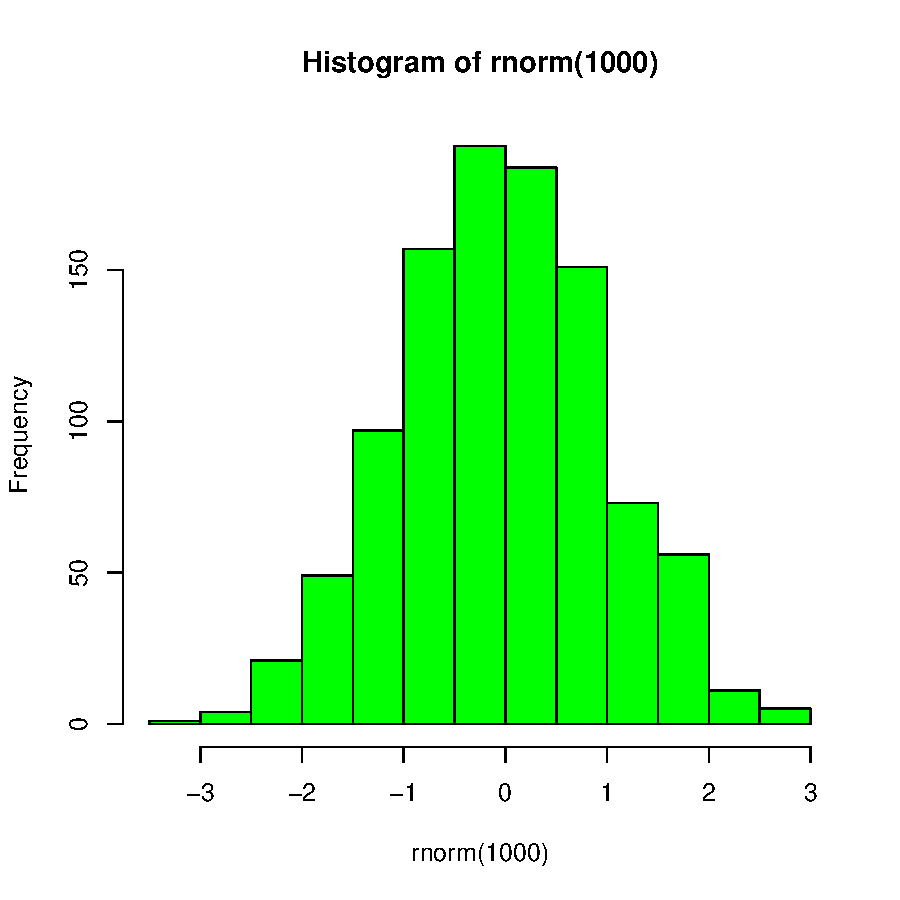
\includegraphics{SummerBridge2-005}
\vspace{0ex}
\vfill
\end{block}
\vfill

%-- Block 3-2
\begin{block}{Prediction Errors}
\vspace{0ex}
\vfill
\end{block}
\vfill

%-- Block 3-3
\begin{block}{Further Directions}
\begin{itemize}
\item Use the models developed in this poster to predict county votes for states that have had similar marriage amendments such as South Carolina, Wisconsin, South Dakota, Florida, Idaho, Alabama, Utah, Michigan, Texas, Arkansas, Louisiana, Kansas, Kentucky, Ohio, and Nebraska. 
\item  Use ensemble methods (combining multiple models) for better prediction.
\item  Make our local maps available via the internet using the shiny server.
\end{itemize}
\vspace{0ex}
\vfill
\end{block}
\vfill

%-- Block 3-4
\begin{block}{References}
\footnotesize
\setbeamertemplate{bibliography item}[text]
\vspace{-1ex}

\bibliographystyle{plain}  % can use plain but comment out natbib at top if using plain
\bibliography{knitr-packages,poster}
\normalsize
\vfill
\end{block} 
\vfill

\end{minipage}
\end{column}%3




\end{columns}
\end{frame}
\end{document}

